\documentclass[11pt]{article}

\usepackage[margin=0.82in]{geometry}
\usepackage[T1]{fontenc}
\usepackage[utf8]{inputenc}
\usepackage{lmodern}
\usepackage{microtype}
\usepackage{amsmath,amssymb,amsthm,mathtools}
\usepackage{booktabs,tabularx,array,longtable,multirow}
\usepackage{xcolor}
\usepackage{graphicx}
\usepackage{enumitem}
\usepackage{algorithm}
\usepackage{algpseudocode}
\usepackage{siunitx}
\usepackage{tikz}
\usetikzlibrary{arrows.meta,positioning,fit,backgrounds}
\usepackage[numbers,sort&compress]{natbib}
\usepackage{hyperref}
\usepackage[nameinlink,noabbrev]{cleveref}
\usepackage{fancyhdr}
\makeatletter
\renewcommand{\theALG@line}{\thealgorithm.\arabic{ALG@line}}
\providecommand*{\theHALG@line}{}
\renewcommand*{\theHALG@line}{\thealgorithm.\arabic{ALG@line}}
\makeatother

\definecolor{certblue}{HTML}{2455A4}
\definecolor{certgreen}{HTML}{2A7F62}
\definecolor{certorange}{HTML}{D97706}
\definecolor{certred}{HTML}{B42318}
\hypersetup{
  colorlinks=true,
  linkcolor=certblue,
  citecolor=certgreen,
  urlcolor=certblue,
  pdftitle={Proof-Carrying, Model-Aware Compilation of Rigorous Trotter Resource Bounds},
  pdfauthor={Junkai Wang}
}

\pagestyle{fancy}
\fancyhf{}
\fancyhead[L]{Proof-Carrying Trotter Resource Bounds}
\fancyhead[R]{J. Wang}
\fancyfoot[C]{\thepage}
\setlength{\headheight}{14pt}
\setlength{\parindent}{1.25em}
\setlength{\parskip}{0.22em}
\setlength{\emergencystretch}{3em}
\setlist{itemsep=0.25em,topsep=0.35em}

\newtheorem{theorem}{Theorem}[section]
\newtheorem{lemma}[theorem]{Lemma}
\newtheorem{proposition}[theorem]{Proposition}
\newtheorem{corollary}[theorem]{Corollary}
\theoremstyle{definition}
\newtheorem{definition}[theorem]{Definition}
\newtheorem{remark}[theorem]{Remark}

\newcommand{\opnorm}[1]{\left\lVert #1\right\rVert}
\newcommand{\paulinorm}[1]{\left\lVert #1\right\rVert_{1,\mathrm{P}}}
\newcommand{\comm}[2]{\left[#1,#2\right]}
\newcommand{\ad}{\operatorname{ad}}
\newcommand{\eps}{\varepsilon}
\newcommand{\cert}{\textsc{Cert}}
\newcommand{\code}[1]{\texttt{#1}}
\newcommand{\Rge}{R_{\ge 8}}

\title{\textbf{Proof-Carrying, Model-Aware Compilation of\\
Rigorous Trotter Resource Bounds}\\[0.4em]
\large A Machine-Certified $4.050498\times$ Reduction for a\\
Two-Dimensional Heisenberg Benchmark}
\author{Junkai Wang\\
\small WangTheoPhys / Wander Team\\
\small Quantum Circuit Simulation Track\\
\small \href{mailto:WangTheoPhys@outlook.com}{WangTheoPhys@outlook.com}}
\date{July 31, 2026}

\begin{document}
\maketitle
\begin{abstract}
Rigorous product-formula resource estimates often lose most of their useful
model structure before the final norm is evaluated.  We introduce a
proof-carrying, model-aware compiler that delays norm inequalities while
translating a product formula through four intermediate representations:
sparse free associative words, homogeneous free-Lie defects, concrete
symplectic Pauli ledgers, and exact rational norm certificates.  The compiler
combines identical translated Pauli strings before taking norms and replaces
termwise Pauli-$\ell_1$ estimates by independently verified
pairwise-anticommuting groups whenever possible.  A finite right-logarithmic
generator expansion and an outward-rational geometric tail then convert the
local certificate into a nonasymptotic global error bound and an integer gate
count.

For the periodic $12\times12$ spin-$1/2$ isotropic Heisenberg model at
$T=1$ and global operator-norm tolerance $10^{-6}$, we compare the same four
matching fragments, the same 31-stage five-copy fourth-order Suzuki formula,
and the same compilation cost on both sides.  A pinned interval instantiation
of the Childs--Su--Tran--Wiebe--Zhu high-order commutator theorem requires 393
steps and 11,791 merged group exponentials.  Our certificate accepts 97 steps
and rejects 96, requiring 2,911 groups.  The exact improvement is
$11791/2911=4.050498110614909\ldots$, a 75.3117\% reduction.  The leading D4
sidecar contains 75,324 canonical Pauli terms partitioned into 7,576 verified
anticommuting groups.  The search procedure is outside the trusted computing
base: a smaller verifier rechecks coverage, every anticommutation relation,
outward square-root bounds, the finite-step ledger, the adjacent integer
boundary, and all resource arithmetic.  An exact D5 side study and a
quantitative fivefold feasibility audit are reported separately; no 78-step
global certificate is claimed.
\end{abstract}

\noindent\textbf{Keywords:} Hamiltonian simulation; Trotter--Suzuki product
formulas; rigorous error bounds; Pauli algebra; computer-assisted proof;
quantum resource estimation.

\tableofcontents
\clearpage

\section{Introduction}
\label{sec:introduction}

Product formulas remain among the most transparent constructions for digital
Hamiltonian simulation.  If $H=\sum_{\gamma=1}^{\Gamma}H_\gamma$, a product
formula replaces $\exp(-itH)$ by a sequence of exponentials of simpler
fragments $H_\gamma$.  The method needs no block encoding, can preserve the
geometry of local interactions, and maps naturally to hardware with limited
connectivity.  Its practical cost, however, is determined not merely by its
formal order but by the constant in a rigorous finite-time error bound.  A
factor lost in this constant is amplified when the bound is inverted to select
an integer number of Trotter steps and then multiplied by every local
propagator in every step.

The modern commutator-scaling theory of Childs, Su, Tran, Wiebe, and Zhu
provides a general foundation for such estimates
\cite{childs2021trotter}.  It replaces purely norm-sum scaling by sums of
nested commutators and thereby exploits locality and exact commutation.  This
framework is sufficiently general to cover arbitrary order and many
Hamiltonian classes, but a general theorem must remain conservative about the
concrete algebra of a fixed model.  In a Pauli lattice, multiple formal
commutator paths may evaluate to the same operator with opposite signs;
translation-equivalent terms may repeat; and distinct surviving Paulis may
anticommute, so their sum has a Euclidean rather than taxicab norm.  Applying a
triangle inequality before these facts become visible irreversibly discards
them.

This paper studies the resulting ``last-mile'' problem:

\begin{quote}
Given a fixed local Hamiltonian, fragmentation, product formula, simulation
time, error tolerance, and compilation model, how can one automatically
produce a tighter \emph{machine-checkable} worst-case resource bound without
changing the target quantum circuit family?
\end{quote}

Our answer is to treat error analysis as compilation.  The source program is
the Hamiltonian and product formula.  The compiler lowers it through
successive algebraic intermediate representations, performs semantics-
preserving optimization passes, and emits a proof object.  In contrast with a
normal circuit optimizer, the principal output is not a different sequence of
quantum gates.  It is a smaller certified number of repetitions of the same
sequence.  The design follows a proof-carrying principle: expensive symbolic
search may be heuristic, but an accepted result must carry all data required
for a simpler independent verifier to reconstruct the logical obligations.

\subsection{Contributions}

The main contributions are as follows.

\begin{enumerate}
\item \textbf{A multi-representation error compiler.}  We compute the
  truncated logarithm of the complete product formula in a sparse free
  associative algebra, project its homogeneous defects to free-Lie elements,
  evaluate those elements in a concrete symplectic Pauli representation, and
  finally emit exact rational certificate data.  Each lowering step has an
  explicit invariant and can be checked independently.

\item \textbf{Norm-last concrete evaluation.}  We canonicalize finite Pauli
  configurations under lattice translation and combine identical Pauli
  strings with exact coefficients before applying a final norm inequality.
  This reverses the conventional expand-and-bound order and preserves
  cancellations that are invisible at the level of abstract support counts.

\item \textbf{Certified anticommuting norm compression.}  We construct a
  graph whose vertices are leading-defect Pauli terms and whose edges encode
  anticommutation.  An untrusted search partitions terms into pairwise-
  anticommuting groups.  The certificate records the full partition and
  outward rational square-root bounds; the verifier rechecks exact coverage
  and every edge used.  For the principal instance, this lowers the D4
  translation-cell bound from 20.160968407335066 to 6.472926505087888.

\item \textbf{A nonasymptotic right-generator closure.}  We convert the
  degree-five and degree-seven logarithmic defects into the right logarithmic
  generator, retain degrees D4 through D7, use a Heisenberg-specific local
  commutator lemma, and control all remaining degrees by a rational geometric
  locality tail.  Thus the resource result does not rely on leading-order
  extrapolation.

\item \textbf{An independently reproducible finite-instance result.}  For a
  $12\times12$ periodic Heisenberg lattice, the certificate accepts 97 steps
  and rejects 96.  Relative to a pinned 393-step instantiation of the
  published high-order theorem, this reduces merged group exponentials from
  11,791 to 2,911.  A fast verifier, deep regeneration mode, small-system
  dense cross-check, mutation tests, and a SHA-256 manifest support the claim.
\end{enumerate}

\subsection{Scope and nonclaims}

The result is a finite-size constant-factor improvement, not a new asymptotic
Hamiltonian-simulation complexity.  It applies to a uniform operator-norm
guarantee for a fixed deterministic product formula.  Methods based on low-
energy inputs, average-case norms, multi-product formulas, linear combinations
of unitaries, extrapolation, or stochastic compensation solve different
resource problems and may achieve stronger precision scaling under their own
cost models.  We compare these directions in \cref{sec:related} but do not
rank incomparable gate counts as a single global record.

The exact D5 side study and the $r=78$ arithmetic indicate a possible
fivefold threshold.  They do not establish it.  Throughout this manuscript,
``certified'' refers only to statements accepted by the supplied rational
certificate and verifier.  Numerical dense simulation is used solely as a
cross-check, and conditional research estimates are labeled explicitly.

\section{Problem Formulation and Fixed Benchmark}
\label{sec:problem}

\subsection{Hamiltonian and fragmentation}

Let $\Lambda=(\mathbb{Z}/L\mathbb{Z})^2$ be a periodic square lattice with one
qubit per site.  The target Hamiltonian is
\begin{equation}
 H=\sum_{\langle u,v\rangle}h_{uv},\qquad
 h_{uv}=\frac{X_uX_v+Y_uY_v+Z_uZ_v}{4}.
 \label{eq:hamiltonian}
\end{equation}
Horizontal and vertical bonds are split by parity into four perfect
matchings $M_1,\ldots,M_4$.  Defining
$H_a=\sum_{(u,v)\in M_a}h_{uv}$ gives
$H=H_1+H_2+H_3+H_4$.  Terms within each matching have disjoint support and
therefore commute exactly.  For real-time analysis we use anti-Hermitian
generators $A_a=-iH_a$ and $A=\sum_a A_a$.

The principal benchmark fixes
\begin{equation}
 L=12,qquad N=L^2=144,qquad T=1,qquad \eps=10^{-6}.
 \label{eq:benchmark}
\end{equation}
The required guarantee is uniform over all input states:
\begin{equation}
 \opnorm{e^{-iTH}-\widetilde U_r(T)}\le \eps,
 \label{eq:uniformerror}
\end{equation}
where $\opnorm{\cdot}$ is the spectral norm.  This is deliberately stronger
than an observable-specific, state-dependent, or average-case condition.

\subsection{Product formula}

Let $S_2(t)$ denote the symmetric second-order formula for the four fragments.
The standard five-copy Suzuki recursion \citep{suzuki1991general} forms
\begin{equation}
 S_4(t)=S_2(pt)^2S_2((1-4p)t)S_2(pt)^2,\qquad
 p=(4-4^{1/3})^{-1}.
 \label{eq:suzuki4}
\end{equation}
After merging adjacent equal fragments, one step contains 31 group
exponentials.  The $r$-step approximation is
\begin{equation}
 \widetilde U_r(T)=S_4(T/r)^r.
\end{equation}
The baseline and candidate use precisely the same ordered stage sequence and
the same outward interval for the algebraic coefficient $p$.  Consequently,
any reduction in $r$ is a proof improvement rather than a change of
simulation formula.

\subsection{Cost model}

Equal fragments at the boundary between adjacent symmetric steps merge.  The
first step contributes 31 groups and each additional step contributes 30:
\begin{equation}
 G(r)=31+30(r-1)=30r+1.
 \label{eq:groups}
\end{equation}
Each perfect matching contains $N/2=72$ disjoint bonds.  We therefore count
\begin{equation}
 B(r)=72G(r)
 \label{eq:bonds}
\end{equation}
bond propagators.  Using the same conservative upper bound of three CNOTs per
normalized Heisenberg bond propagator on both sides gives
\begin{equation}
 C(r)\le 3B(r)=216G(r).
 \label{eq:cnots}
\end{equation}
The primary ratio is identical for groups, bond propagators, and this CNOT
upper bound because the multiplicative factors cancel.

\subsection{Compiler contract}

The compiler receives a tuple
\begin{equation}
 \mathcal I=(H,\mathcal F,S,T,\eps,\mathcal C),
\end{equation}
where $\mathcal F$ is a fragmentation, $S$ a product formula, and
$\mathcal C$ a cost model.  It must return a tuple
\begin{equation}
 \mathcal O=(r_\star,E_{r_\star},E_{r_\star-1},R_\star,\cert),
\end{equation}
such that an independent verifier establishes
\begin{align}
 E_{r_\star}&\le\eps,& E_{r_\star-1}&>\eps,\label{eq:adjacent}\
 R_\star&=\mathcal C(S,r_\star),
\end{align}
using exact integers, rational numbers, or outward rational intervals.  The
second inequality does not prove that the physical circuit with
$r_\star-1$ fails; it proves that $r_\star$ is the smallest integer accepted
by this particular certified upper-bound function.  This distinction is
retained throughout.

\section{Reconstructing the Published-Theorem Baseline}
\label{sec:baseline}

The phrase ``published baseline'' can obscure two logically distinct objects.
The first is the high-order commutator theorem published by Childs et al.
\cite{childs2021trotter}; the second is our fixed, machine-evaluated
instantiation of that theorem.  The number 393 is not a table entry quoted
from the 2021 paper.  It is obtained by applying the published framework to
\cref{eq:hamiltonian,eq:benchmark,eq:suzuki4} with a specified norming and
interval procedure.  We call it the \emph{pinned control}.

\subsection{Expansion-first local norming}

The high-order theorem represents product-formula error by partial sums and
nested commutators.  For the pinned control, every partial matching sum is
expanded into local Heisenberg bonds, zero commutators are removed, and each
surviving concrete Pauli expansion is bounded by its Pauli-$\ell_1$ norm.
The resulting site-density upper bound is stored as an exact rational number
whose outward decimal is
\begin{equation}
 \alpha_{\mathrm{base}}\le164.9759169527440.
\end{equation}
The calculation contains 8,316 theorem terms and 1,024 expanded commutator
keys.  All algebraic product-formula coefficients are enclosed by rational
intervals; no rounded decimal is used as the source of the result.

The theorem admits a discrete family of center choices controlling how the
high-order integral representation is partitioned.  We evaluate all 31
admissible centers.  Center 20 gives the smallest certified control, and
inverting its global bound at tolerance $10^{-6}$ yields
\begin{equation}
 r_{\mathrm{base}}=393,\qquad G(r_{\mathrm{base}})=11{,}791.
\end{equation}
The main certificate stores both the exact site-density rational and the
chosen center.  A deep verification mode regenerates the center scan rather
than trusting these stored labels.

\subsection{Where the baseline loses information}

The baseline is rigorous, general, and already exploits exact commutation.
Its looseness in this instance arises from the order of operations.  Once an
abstract contribution is replaced by an independent positive norm, later
knowledge cannot recover cancellation between that contribution and another
one.  Four losses are particularly important:

\begin{enumerate}
\item distinct free words can map to the same nested-commutator or Pauli
  contribution with opposite signs;
\item distinct translated local clusters can share a canonical translation
  representative;
\item different commutator paths can produce exactly the same Pauli string;
\item different surviving Pauli strings can anticommute, causing cross terms
  to vanish when the group norm is squared.
\end{enumerate}

The proposed compiler postpones the irreversible inequality until these
relations have been exposed.  Importantly, it does not treat the baseline as
incorrect.  It constructs a stronger proof for the same circuit and then
verifies both sides under a common benchmark and cost model.

\begin{table}[t]
\centering
\caption{Logical separation between the published theorem and the pinned
finite-instance control.}
\label{tab:baseline-separation}
\begin{tabularx}{\textwidth}{@{}lXX@{}}
\toprule
 & Published theory & Pinned control used here \\
\midrule
Source & Childs et al. commutator-scaling framework & Exact interval
instantiation for the fixed Heisenberg benchmark \\
Scope & General Hamiltonian fragments and formula order & $L=12$, four
matchings, five-copy $S_4$, $T=1$, $\eps=10^{-6}$ \\
Norming & Theorem permits commutator-sensitive evaluation & Expanded local
Pauli-$\ell_1$ procedure fixed by the certificate \\
Finite number & No published 393-step table entry & 31 centers scanned;
center 20 yields 393 steps \\
Role & Mathematical foundation & Auditable comparison control \\
\bottomrule
\end{tabularx}
\end{table}

\section{A Proof-Carrying Compiler for Error Bounds}
\label{sec:compiler}

\subsection{Intermediate representations}

The compiler is organized around four intermediate representations (IRs).
The \emph{word IR} stores sparse homogeneous polynomials in noncommuting
letters $A_1,\ldots,A_4$.  The \emph{Lie IR} stores homogeneous logarithmic
defects as rational linear combinations of right-nested commutators.  The
\emph{Pauli IR} stores canonical finite-support symplectic Pauli strings with
exact coefficients per translation cell.  The \emph{certificate IR} stores
partitions, rational norm enclosures, finite-step contributions, tail data,
hash bindings, and resource arithmetic.

\begin{figure}[t]
\centering
\resizebox{\textwidth}{!}{%
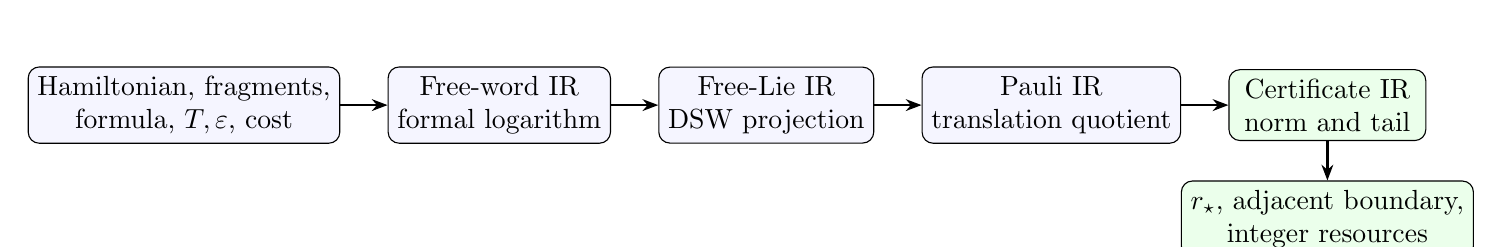
\begin{tikzpicture}[
 node distance=5mm and 6mm,
 box/.style={draw,rounded corners,align=center,minimum height=8mm,minimum width=25mm,fill=blue!4},
 certbox/.style={box,fill=green!8},
 arr/.style={-{Stealth[length=2mm]},thick}
]
\node[box] (input) {Hamiltonian, fragments,\\formula, $T,\eps$, cost};
\node[box,right=of input] (word) {Free-word IR\\formal logarithm};
\node[box,right=of word] (lie) {Free-Lie IR\\DSW projection};
\node[box,right=of lie] (pauli) {Pauli IR\\translation quotient};
\node[certbox,right=of pauli] (cert) {Certificate IR\\norm and tail};
\node[certbox,below=of cert] (output) {$r_\star$, adjacent boundary,\\integer resources};
\draw[arr] (input)--(word);
\draw[arr] (word)--(lie);
\draw[arr] (lie)--(pauli);
\draw[arr] (pauli)--(cert);
\draw[arr] (cert)--(output);
\end{tikzpicture}
}
\caption{Compiler pipeline.  Algebraic structure is retained until the Pauli
IR; irreversible norm inequalities enter only in the certificate IR.}
\label{fig:pipeline}
\end{figure}

Each lowering pass preserves a semantic invariant.  Word multiplication
preserves the truncated product series.  Formal logarithms preserve the
truncated exponential identity.  DSW projection preserves the homogeneous
Lie element.  Pauli evaluation is a representation homomorphism.  Translation
canonicalization preserves the sum per cell.  Exact aggregation preserves the
represented operator.  Finally, grouped norming replaces equality by a
verified upper bound.

\subsection{End-to-end algorithm}

\begin{algorithm}[t]
\caption{Compile a product formula into a resource certificate}
\label{alg:compiler}
\begin{algorithmic}[1]
\Require $(H,\mathcal F,S,T,\eps,\mathcal C)$ and truncation policy
\Ensure Certificate accepted by an independent verifier
\State parse all stage coefficients into exact algebraic or outward intervals
\State $P(t)\gets$ truncated free-word expansion of the complete stage product
\State $L(t)\gets\log P(t)$ in the sparse free associative algebra
\State verify order conditions and time-reversal parity through target degree
\For{$d\in\{5,7\}$}
  \State $E_d\gets$ DSW projection of the homogeneous component $L_d$
  \State $Q_d\gets$ evaluate $E_d$ in the concrete local Pauli representation
  \State quotient $Q_d$ by translation and combine identical Pauli strings
\EndFor
\State discover weighted pairwise-anticommuting groups for the leading ledger
\State emit full group membership and outward rational square-root bounds
\State convert $E_5,E_7$ to right-generator terms D4--D7
\State close all remaining terms with a rational locality majorant and tail
\State find the smallest integer $r_\star$ whose certified bound is at most $\eps$
\State compile $r_\star$ to groups, bond propagators, and CNOT upper bound
\State emit hashes, provenance, and adjacent-step evidence
\end{algorithmic}
\end{algorithm}

The algorithm intentionally separates \emph{discovery} from \emph{trust}.
The formal-series generator and grouping search can be large and optimized for
throughput.  Their output is not accepted because the code ran successfully;
it is accepted only after a second path rechecks the certificate.  In
particular, no claim depends on the greedy grouping being optimal.  Any valid
partition gives a sound bound, and a better heuristic can improve the bound
without expanding the trusted computing base.

\subsection{What is improved at each pass}

\begin{table}[t]
\centering
\caption{Compiler passes and the information they preserve.}
\label{tab:passes}
\begin{tabularx}{\textwidth}{@{}p{0.19\textwidth}p{0.26\textwidth}Xp{0.18\textwidth}@{}}
\toprule
Pass & Conventional relaxation & Replacement & Verified invariant \\
\midrule
Complete formula log & Bound stages or partial sums separately & Multiply all
stages and take the formal log before norming & Truncated series identity and
order conditions \\
Lie projection & Treat free words as unrelated monomials & Project homogeneous
log defects into free-Lie elements & DSW identity at fixed degree \\
Concrete evaluation & Count generic nonzero commutators & Evaluate exact local
Pauli products and phases & Symplectic multiplication and support \\
Translation quotient & Count translated clusters separately & Select a
canonical orbit representative & Translation-equivalent configurations merge \\
Coefficient aggregation & Take absolute values by derivation path & Sum exact
coefficients of identical Paulis & Operator represented by sparse ledger \\
Anticommuting grouping & Apply termwise Pauli-$\ell_1$ & Use exact group
$\ell_2$ identities & Coverage and pairwise anticommutation \\
Finite-step closure & Use only leading order & Retain D4--D7 and rational tail
& Global error upper bound \\
Adjacent integer search & Round a continuous estimate & Verify $r$ and $r-1$
exactly & Smallest integer accepted by this bound \\
\bottomrule
\end{tabularx}
\end{table}

This organization also answers how the method should be extended.  A new
Hamiltonian needs a representation backend and local-support rules; a new
formula needs a stage generator and exact coefficient enclosure; a new norm
strategy needs a certificate schema and verifier.  The higher layers need not
be rewritten if their interfaces and invariants remain unchanged.

\section{Complete-Formula Free-Lie Extraction}
\label{sec:free-lie}

The first source of slack in a generic product-formula estimate is often not
the inequality used at the end, but the loss of cancellation before the
inequality is applied.  We therefore expand the \emph{complete} 31-stage
formula as one formal object.  This section describes the representation and
the identities checked by the implementation.

\subsection{Sparse truncated words}

Let $\mathbb{K}\langle A_1,\ldots,A_m\rangle$ denote the free associative
algebra over a coefficient field $\mathbb K$.  A homogeneous word
$w=(j_1,\ldots,j_d)$ represents $A_{j_1}\cdots A_{j_d}$.  Up to degree $q$,
we store a series as the sparse map
\begin{equation}
  P(t)=1+\sum_{d=1}^{q}t^d\sum_{|w|=d}p_w w+O(t^{q+1}).
  \label{eq:sparse-word-series}
\end{equation}
Multiplication is truncated convolution.  An exponential stage is generated
by
\begin{equation}
  \exp(a t A_j)=\sum_{k=0}^{q}\frac{(a t)^k}{k!}A_j^k+O(t^{q+1}),
\end{equation}
and all 31 stages are multiplied in their actual execution order.  The
coefficients $a$ are held as outward rational intervals.  Thus every stored
coefficient encloses the corresponding real algebraic coefficient, including
the fourth-order Suzuki coefficient involving $4^{1/3}$.

For $X=P-1$, the formal logarithm is
\begin{equation}
  \log P=\sum_{k=1}^{q}\frac{(-1)^{k+1}}{k}X^k+O(t^{q+1}).
  \label{eq:formal-log}
\end{equation}
No matrices and no floating-point eigensolvers enter this computation.  The
calculation is universal in the letters; only after the Lie defect is known do
we substitute the concrete Heisenberg fragments.

\subsection{Order, symmetry, and the full-stage cancellation budget}

Write the ideal generator as $A=\sum_{j=1}^{4}A_j$ and the logarithm of a
single formula step as
\begin{equation}
  \log S_4(t)=tA+t^5E_5+t^7E_7+O(t^9).
  \label{eq:symmetric-log}
\end{equation}
Fourth order requires the degree-two through degree-four defects to vanish.
Time symmetry, $S_4(-t)=S_4(t)^{-1}$, implies that the logarithm is odd, so its
even homogeneous components vanish.  The compiler checks these statements
coefficient by coefficient in the word IR; it does not infer them merely from
the name of the formula.

This global construction matters.  If a bound is applied to each stage or to
each recursive subformula before the product is assembled, opposite
coefficients and Jacobi-related terms can no longer cancel.  In our pipeline,
absolute values first appear only after the complete formula has been
projected, evaluated, translated, and aggregated.  This ordering of
operations is the main methodological distinction from a direct
``expand--triangle-inequality'' instantiation of a general commutator theorem.

\subsection{Dynkin--Specht--Wever projection}

The homogeneous component $L_d$ of a logarithm of group-like series is a Lie
element.  We use the Dynkin--Specht--Wever (DSW) map to expose that structure.
For a word $w=x_1\cdots x_d$, define
\begin{equation}
  D(w)=[x_1,[x_2,\ldots,[x_{d-1},x_d]\ldots]].
\end{equation}
The DSW theorem gives $D(L_d)=dL_d$ for homogeneous Lie elements
\citep{reutenauer1993free}.  Consequently,
\begin{equation}
  E_d=L_d=\frac{1}{d}\sum_{|w|=d}\ell_w D(w),
  \label{eq:dsw}
\end{equation}
where $\ell_w$ are the word coefficients obtained from \cref{eq:formal-log}.
Equation~\eqref{eq:dsw} is used as a projection and as an independently
checkable identity: expanding its right-hand side back into words must recover
$L_d$ interval-wise.

\begin{proposition}[Semantic preservation of the Lie lowering pass]
\label{prop:lie-pass}
Assume the input interval map encloses every coefficient of the degree-$d$
homogeneous formal logarithm and the DSW reconstruction check succeeds.  Then
the emitted nested-commutator interval map encloses the exact homogeneous Lie
defect $E_d$.
\end{proposition}

\begin{proof}
The DSW map is linear over the coefficient field.  Interval scalar
multiplication and addition are inclusion isotone, so applying $D/d$ to the
input enclosures contains its application to the exact coefficients.  The DSW
identity fixes the exact image to $E_d$.  The reconstruction check additionally
guards against word-order, sign, and truncation errors in the implementation.
\end{proof}

\subsection{Why this is an algorithmic improvement}

The free-Lie stage is not a new product formula: it is a better compiler for a
fixed formula.  Its improvement is threefold.  First, it preserves
cross-stage cancellations.  Second, it replaces derivation histories by a
canonical operator expression.  Third, it makes the later model substitution
sparse: nested commutators that vanish under the local Pauli representation
are removed exactly rather than charged by a worst-case commutator factor.
The cost is an offline symbolic calculation whose size grows rapidly with
degree.  That cost is acceptable here because the certificate is generated
once and verified much more cheaply than it is discovered.

\section{Concrete Pauli Evaluation and Translation Quotienting}
\label{sec:pauli}

After free-Lie extraction, the compiler substitutes the four checkerboard
fragments of the square-lattice Heisenberg Hamiltonian.  This is the point at
which generic commutator counting is replaced by exact model algebra.

\subsection{Symplectic Pauli representation}

Ignoring a separately stored phase, an $n$-qubit Pauli is represented by two
bit strings $(x,z)\in\mathbb F_2^{2n}$ through the stabilizer/symplectic
formalism \citep{gottesman1997stabilizer},
$P=i^\kappa X^xZ^z$.  Multiplication is bitwise xor plus an exactly updated
phase.  Two Paulis commute exactly when their symplectic product vanishes:
\begin{equation}
  [P(x,z),P(x',z')]=0
  \quad\Longleftrightarrow\quad
  x\!\cdot\!z'+z\!\cdot\!x'=0\pmod 2.
  \label{eq:symplectic-commutation}
\end{equation}
Thus a nested commutator is evaluated without constructing a
$2^{144}\times2^{144}$ matrix.  At each bracket, commuting pairs are deleted;
anticommuting pairs produce the exact factor and phase.  Duplicate bit strings
are combined before the next bracket.

The local bond operator
\begin{equation}
 h_{uv}=\frac14(X_uX_v+Y_uY_v+Z_uZ_v)
 \label{eq:bond-hamiltonian}
\end{equation}
has only three Pauli summands.  Each of the four fragments is a sum over a
perfect matching of the periodic $12\times12$ lattice.  Terms within a
matching commute and their exponentials reduce to independent two-qubit bond
propagators.

\subsection{Locality before enumeration}

The support of $[P,Q]$ is contained in
$\operatorname{supp}(P)\cup\operatorname{supp}(Q)$, and the bracket vanishes
when the strings commute.  The implementation therefore carries connected
bond clusters rather than global lattice objects.  A degree-$d$ nested
commutator can touch only a bounded neighborhood of its seed bond.  Candidate
bonds outside that neighborhood are never enumerated.  This converts a
nominally exponential global construction into a finite local calculation
followed by a translation-density factor.

For the $L=12$ benchmark the supports fit inside the injectivity radius of the
torus for the degrees used in the explicit ledger.  Periodic coordinates are
nevertheless retained, and wraparound is checked rather than assumed away.
This avoids silently importing an infinite-lattice result into a finite
periodic instance.

\subsection{Canonical translation representatives}

Let $\tau_a$ translate a Pauli string by a lattice displacement $a$.  We
choose the lexicographically least serialization among all translates as the
orbit representative
\begin{equation}
  \operatorname{can}(P)=\min_{a\in\mathbb Z_L^2}\operatorname{serialize}(\tau_aP).
  \label{eq:translation-canonical}
\end{equation}
The coefficient map is then aggregated by this key.  Canonicalization occurs
before taking absolute values, so translated derivation paths that land on the
same physical Pauli can cancel exactly.

\begin{proposition}[Correctness of translation aggregation]
\label{prop:translation}
Let $Q=\sum_jc_jP_j$ be a translation-invariant operator written with a marked
origin, and let $\bar c_P$ be the sum of all coefficients mapped to canonical
representative $P$.  On an $L\times L$ periodic lattice,
\begin{equation}
  Q=\sum_{a\in\mathbb Z_L^2}\tau_a
      \left(\sum_{P}\bar c_P P\right),
\end{equation}
with the conventional stabilizer multiplicities included in $\bar c_P$.
\end{proposition}

\begin{proof}
Translation partitions the enumerated terms into disjoint group orbits.
Within each orbit, linearity permits coefficient aggregation at a selected
representative.  Re-expanding the orbit sum recovers every translated term
with the same multiplicity.  The implementation records orbit and stabilizer
counts, making the equality a finite combinatorial check.
\end{proof}

\subsection{Exact aggregation and interval coefficients}

Every coefficient is an interval $[c^-,c^+]$ with rational endpoints.  When
multiple derivation paths yield the same Pauli key, intervals are added first.
Only then is an outward absolute upper bound formed:
\begin{equation}
  |[c^-,c^+]|_\uparrow=\max\{|c^-|,|c^+|\}.
\end{equation}
This order is essential.  Replacing $\sum_jc_j$ by $\sum_j|c_j|$ earlier would
discard the formula-specific and model-specific cancellations that the
compiler was designed to retain.

The output of this pass is not merely a scalar norm.  It is a complete sparse
ledger of canonical Pauli keys and coefficient enclosures.  That ledger can be
hashed, independently replayed, regrouped by a future heuristic, or sampled
for direct small-system matrix cross-checks.  These properties turn a
one-off symbolic calculation into reusable evidence.

\section{Anticommuting Norm Certificates}
\label{sec:norm}

After exact coefficient aggregation, the direct Pauli triangle inequality
$\opnorm{\sum_j c_jP_j}\leq\sum_j|c_j|$ remains sound but unnecessarily loose.
The leading right-generator defect contains many mutually anticommuting
strings.  Their norm is an $\ell_2$, not an $\ell_1$, quantity.

\subsection{Weighted anticommuting groups}

\begin{lemma}[Pairwise-anticommuting Pauli norm]
\label{lem:anticommuting}
Let $P_1,\ldots,P_k$ be Hermitian Pauli operators with $P_i^2=I$ and
$\{P_i,P_j\}=0$ for $i\neq j$.  For real coefficients $c_i$,
\begin{equation}
  \opnorm{\sum_{i=1}^{k}c_iP_i}=\sqrt{\sum_{i=1}^{k}c_i^2}.
  \label{eq:anticommuting-norm}
\end{equation}
\end{lemma}

\begin{proof}
Squaring the sum gives
$\sum_i c_i^2I+\sum_{i<j}c_ic_j(P_iP_j+P_jP_i)$; all cross terms vanish.
Hence every eigenvalue has magnitude $\sqrt{\sum_i c_i^2}$, proving the
operator-norm identity.
\end{proof}

For interval coefficients we replace each $|c_i|$ by its outward rational
upper endpoint and enclose the square root from above.  If
$\mathcal G=\{G_1,\ldots,G_s\}$ is a partition of the Pauli ledger into
pairwise-anticommuting groups, the certified cell bound is
\begin{equation}
 B_{\mathcal G}=\sum_{g=1}^{s}
       \sqrt{\sum_{j\in G_g}|c_j|_\uparrow^2}_{\,\uparrow}.
 \label{eq:grouped-bound}
\end{equation}
Singletons are permitted, so the method is never less sound than termwise
norming and can be applied incrementally.

\subsection{Grouping as a graph certificate}

Construct the anticommutation graph whose vertices are canonical Pauli terms
and whose edges join anticommuting pairs.  A valid group is a clique; a valid
certificate is a vertex-disjoint clique cover.  Finding a minimum-weight cover
is difficult and unnecessary for correctness.  The discovery code uses a
deterministic weighted greedy heuristic that prioritizes large coefficients
and inserts a term only when it anticommutes with every current member.

The verifier does not trust the heuristic.  For every emitted group it checks:
\begin{enumerate}
  \item each referenced Pauli key exists in the coefficient ledger;
  \item every key appears exactly once across the partition;
  \item all distinct pairs satisfy \cref{eq:symplectic-commutation} with
        symplectic parity one;
  \item the squared-weight sum uses the declared coefficient enclosures; and
  \item the rational square-root endpoint squares to at least that sum.
\end{enumerate}
These checks are polynomial in the output size and make optimality irrelevant
to the trusted claim.

\subsection{Leading-defect certificate}

For the degree-four right-generator contribution D4, the concrete ledger has
$75{,}324$ canonical terms.  The emitted partition contains $7{,}576$ groups,
with maximum group size ten.  The resulting per-cell upper bound is
\begin{equation}
  B_{D4}^{\mathrm{group}}=6.472926505087888,
\end{equation}
whereas direct post-aggregation Pauli-$\ell_1$ norming gives
$20.160968407335066$.  The local norm reduction is therefore
$3.114660484942633\times$.  These are certificate statistics, not estimates
from sampled matrices.

\begin{figure}[t]
  \centering
  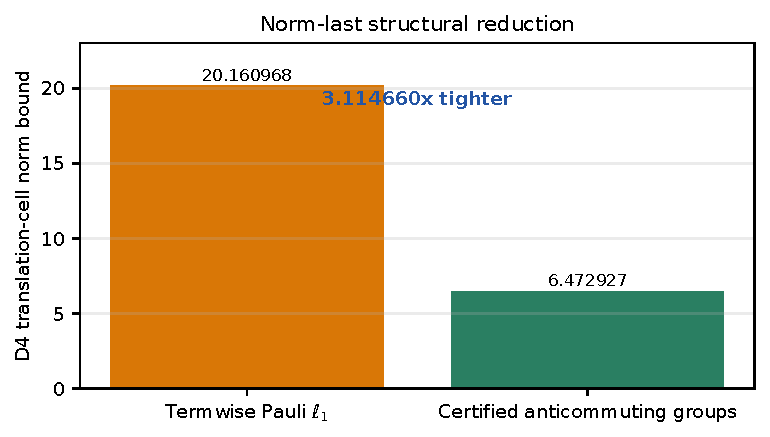
\includegraphics[width=0.68\textwidth]{figures/d4_norm.pdf}
  \caption{Leading D4 cell norm under direct Pauli-$\ell_1$ norming and the
  verified pairwise-anticommuting partition.  Both values are computed after
  exact aggregation; the grouped bar is a rigorous upper bound.}
  \label{fig:d4-norm}
\end{figure}

\subsection{A local Heisenberg identity}

The grouping strategy is reinforced by a small exact algebraic fact.  Let
$h=(XX+YY+ZZ)/4$ on two qubits and let $P$ be a two-qubit Pauli.  Terms of $h$
that commute with $P$ do not contribute to $[h,P]$.  The remaining Pauli
products occur with exactly tracked phases and are pairwise anticommuting for
the local cases used by the certificate.  Consequently the commutator norm is
obtained from a short Euclidean coefficient vector rather than by repeatedly
using $\opnorm{[A,B]}\leq2\opnorm A\opnorm B$.

This lemma is checked exhaustively over the 16 local Paulis.  It supplies an
independent local cross-check on the symplectic engine and explains why the
concrete Heisenberg algebra is substantially smaller than a generic nested
commutator count.  It does not, by itself, prove the global bound; that role is
played by the complete group membership file and finite-step ledger.

\section{Finite-Step Right-Generator Certificate}
\label{sec:finite-step}

An asymptotic statement $O(t^5)$ is insufficient at the target tolerance.
The certified step count is obtained from a finite-$t$ right-generator bound,
including explicit subleading terms and a rational tail.

\subsection{From logarithmic defect to right generator}

Let $S(t)$ denote one formula step and define its right generator
\begin{equation}
  K(t)=S'(t)S(t)^{-1}.
  \label{eq:right-generator}
\end{equation}
For $Z(t)=\log S(t)$, differentiation of the exponential gives
\begin{equation}
  K(t)=\operatorname{dexp}_{Z(t)}(Z'(t))
      =\sum_{n\geq0}\frac{1}{(n+1)!}\ad_{Z(t)}^n Z'(t).
  \label{eq:dexp}
\end{equation}
Substituting \cref{eq:symmetric-log} and collecting powers yields
\begin{equation}
  K(t)-A=t^4D_4+t^5D_5+t^6D_6+t^7D_7+R_{\geq8}(t),
  \label{eq:right-ledger}
\end{equation}
where, writing $B=E_5$ and $C=E_7$, the exact coefficients through degree
seven are
\begin{align}
 D_4&=5B, &
 D_5&=2[A,B],\\
 D_6&=7C+\tfrac23[A,[A,B]], &
 D_7&=3[A,C]+\tfrac16[A,[A,[A,B]]].
\end{align}
The implementation derives these coefficients from the truncated series
rather than trusting the printed display.  The identity clarifies why an
exact leading logarithmic coefficient is not yet a global error certificate:
commutators generated by the differential of the exponential contribute at
the next powers.

\subsection{Duhamel conversion to global error}

Let $U(t)=e^{tA}$ in anti-Hermitian convention.  Variation of constants gives
the one-step estimate
\begin{equation}
 \opnorm{S(\delta)-U(\delta)}
 \leq \int_0^\delta \opnorm{K(s)-A}\,ds.
 \label{eq:one-step-duhamel}
\end{equation}
Unitary telescoping over $r$ equal steps, with $\delta=T/r$, then yields
\begin{equation}
 \opnorm{S(T/r)^r-U(T)}
 \leq r\int_0^{T/r}\opnorm{K(s)-A}\,ds.
 \label{eq:global-duhamel}
\end{equation}
Combining \cref{eq:right-ledger,eq:global-duhamel}, a certificate with norm
upper bounds $b_j\geq\opnorm{D_j}$ and a nonnegative tail majorant $\rho(s)$
establishes
\begin{equation}
 \mathcal E(r)=
 r\left(\sum_{j=4}^{7}\frac{b_j}{j+1}
                  \left(\frac{T}{r}\right)^{j+1}
 +\int_0^{T/r}\rho(s)\,ds\right).
 \label{eq:finite-step-bound}
\end{equation}
All quantities in the machine certificate are rationals.  Decimal values in
this paper are outward-rounded summaries only.

\subsection{Rational tail closure}

The exact ledger is stopped after D7.  Higher degrees are bounded by a
geometric majorant derived from the absolute stage coefficients and local
commutator growth.  In abstract form, if the degree-$k$ coefficient is at most
$M q^{k-k_0}$ for $0\leq q s<1$, then
\begin{equation}
 \rho(s)\leq \frac{M s^{k_0}}{1-qs}.
 \label{eq:geometric-tail}
\end{equation}
The verifier checks the rational preconditions, including positivity of the
denominator on $[0,T/r]$, and integrates an outward upper enclosure.  This is
deliberately more conservative than extrapolating the observed low-degree
coefficients.  It ensures that no uncomputed term is silently discarded.

\begin{theorem}[Soundness of an accepted finite-step certificate]
\label{thm:soundness}
Suppose the verifier accepts (i) interval enclosures for D4--D7, (ii) a valid
operator-norm certificate for each declared coefficient, (iii) a tail
majorant satisfying \cref{eq:geometric-tail} on $[0,T/r]$, and (iv) exact
rational evaluation $\mathcal E(r)\leq\eps$.  Then
\begin{equation}
  \opnorm{S(T/r)^r-e^{TA}}\leq\eps.
\end{equation}
\end{theorem}

\begin{proof}
The accepted coefficient and tail checks bound
$\opnorm{K(s)-A}$ term by term on the complete integration interval.
Integrating preserves the inequality.  Equation~\eqref{eq:global-duhamel}
then bounds the global error, and the exact rational comparison with $\eps$
completes the proof.
\end{proof}

\subsection{Adjacent-step minimality under the certified bound}

The search evaluates integers, not a rounded real-valued estimate.  It returns
the least $r$ accepted by \cref{eq:finite-step-bound} and emits the rejected
neighbor.  For this benchmark,
\begin{align}
 \mathcal E(97)&\leq9.958938494314325\times10^{-7}<10^{-6},\\
 \mathcal E(96)&\leq1.050565873970784\times10^{-6}>10^{-6}.
\end{align}
The second inequality says that 96 is not certified by \emph{this bound}; it
does not prove that the physical simulation error at 96 steps exceeds the
tolerance.  This distinction is retained throughout the paper.

\section{Certificate Architecture and Independent Verification}
\label{sec:verification}

Large symbolic calculations are difficult to trust by inspection.  We use a
proof-carrying architecture: discovery may be complex, but the final claim is
accepted only after a narrower verifier rechecks explicit evidence.

\subsection{Trusted and untrusted components}

\begin{figure}[t]
\centering
\resizebox{\textwidth}{!}{%
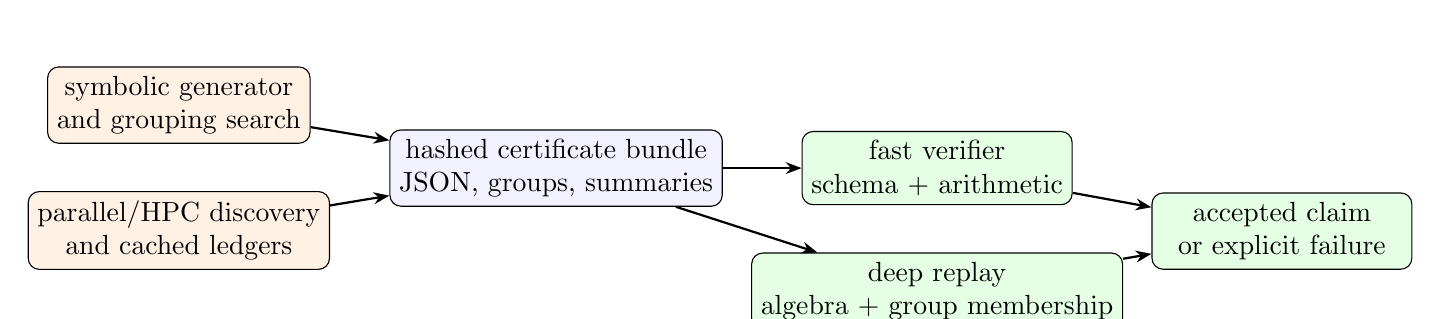
\begin{tikzpicture}[
 node distance=6mm and 10mm,
 box/.style={draw,rounded corners,align=center,minimum height=9mm,minimum width=33mm},
 untrusted/.style={box,fill=orange!10},
 trusted/.style={box,fill=green!10},
 arr/.style={-{Stealth[length=2mm]},thick}
]
\node[untrusted] (gen) {symbolic generator\\and grouping search};
\node[untrusted,below=of gen] (hpc) {parallel/HPC discovery\\and cached ledgers};
\node[box,right=of gen,yshift=-8mm,fill=blue!5] (bundle) {hashed certificate bundle\\JSON, groups, summaries};
\node[trusted,right=of bundle] (fast) {fast verifier\\schema + arithmetic};
\node[trusted,below=of fast] (deep) {deep replay\\algebra + group membership};
\node[trusted,right=of fast,yshift=-8mm] (claim) {accepted claim\\or explicit failure};
\draw[arr] (gen)--(bundle);
\draw[arr] (hpc)--(bundle);
\draw[arr] (bundle)--(fast);
\draw[arr] (bundle)--(deep);
\draw[arr] (fast)--(claim);
\draw[arr] (deep)--(claim);
\end{tikzpicture}
}
\caption{Trust boundary.  Parallel discovery and heuristic grouping are
untrusted producers.  The accepted result depends on explicit evidence and
two verification paths.}
\label{fig:trust-boundary}
\end{figure}

The trusted claim comprises the mathematical lemmas in this paper, the small
verification programs, exact integer/rational arithmetic, and the cryptographic
binding between manifest and sidecars.  It does not require trusting the job
scheduler, the heuristic's optimality, cached stdout, or a claimed successful
HPC run.

\subsection{Certificate contents}

The schema-v3 certificate records:
\begin{itemize}
  \item the complete benchmark tuple, normalization, formula, time, tolerance,
        and primary resource metric;
  \item the pinned theorem instantiation used for the baseline;
  \item coefficient precision policies and rational interval endpoints;
  \item D4 group-certificate path, SHA-256 digest, term count, group count,
        maximum size, and norm enclosure;
  \item D4--D7 and tail contributions at the accepted integer;
  \item the accepted and previous-step global-error rationals;
  \item integer resource arithmetic and the exact improvement ratio; and
  \item auxiliary audit results explicitly separated from the primary claim.
\end{itemize}
Large membership data are sidecars rather than embedded in prose.  The
manifest hash prevents a reviewer from inadvertently validating a different
file with the same name.

\subsection{Fast and deep modes}

Fast verification checks the schema, paths, hashes, integer identities,
rational comparisons, resource formulas, and headline invariants.  It is
intended for continuous integration and reviewer orientation.  Deep
verification additionally replays coefficient aggregation, checks every group
for exact coverage and pairwise anticommutation, verifies all rational square
roots, and reproduces the finite-step sum.

The two modes serve different purposes.  Fast verification answers whether a
checked-in bundle is internally bound and arithmetically self-consistent.
Deep verification answers whether the large algebraic witness supports its
declared norm.  Neither mode treats a rounded decimal in a PDF as evidence.

\subsection{Negative tests and failure localization}

A certificate system is useful only if nearby corruptions fail.  The test
suite mutates representative fields: a group member, a coefficient endpoint,
the accepted step count, a resource total, and a sidecar digest.  Each mutation
must cause a nonzero verifier result.  Further unit tests cover Pauli phase
multiplication, symplectic commutation, periodic canonicalization, rational
square-root enclosure, and the local 16-Pauli lemma.

Failures are reported by layer.  A hash mismatch is distinguished from a
schema error; a duplicate group member from a non-anticommuting pair; a failed
tail precondition from an error-bound comparison.  This makes independent
reproduction tractable: a reviewer need not rerun the entire discovery
pipeline to diagnose a damaged artifact.

\subsection{Claim classes}

We label statements by evidence class:
\begin{description}
  \item[Certified.] Derived from a manifest-bound witness and accepted by the
  verifier, such as the 97-step result and integer resource counts.
  \item[Cross-checked.] Supported by a structurally independent small-system or
  exhaustive local calculation, but not the main large-system proof.
  \item[Conditional.] An arithmetic consequence under a stated future premise,
  such as the norm budget required for a fivefold result.
  \item[Prospective.] A research direction or engineering optimization with no
  claimed current performance.
\end{description}
This vocabulary prevents an observed trend, a possible optimization, and a
completed theorem from being conflated in the abstract or conclusion.

\section{Certified Results}
\label{sec:results}

This section reports only values bound to the checked-in certificate.  The
primary metric is the compiled CNOT upper bound; merged fragment
exponentials and bond propagators are reported because they make the integer
cost model transparent.

\subsection{Headline resource reduction}

The candidate certificate accepts $r=97$ steps.  Adjacent identical fragment
exponentials merge across recursive boundaries, so a 31-stage step sequence
contains
\begin{equation}
  G(r)=30r+1
  \label{eq:merged-groups}
\end{equation}
merged group exponentials.  Each group is one perfect matching with 72 bonds.
The selected two-qubit bond-propagator compilation is charged at three CNOTs.
Therefore
\begin{equation}
  B(r)=72G(r),\qquad C(r)=3B(r)=216G(r).
  \label{eq:resource-map}
\end{equation}

\begin{table}[t]
\centering
\caption{Certified resource comparison under the common compilation model.}
\label{tab:headline-results}
\begin{tabular}{@{}lrrrr@{}}
\toprule
Method & Steps & Merged groups & Bond propagators & CNOT upper \\
\midrule
Pinned published-theorem control & 393 & 11,791 & 848,952 & 2,546,856 \\
Proof-carrying model-aware bound & 97 & 2,911 & 209,592 & 628,776 \\
\midrule
Candidate/control & 0.2468 & 0.2469 & 0.2469 & 0.2469 \\
\bottomrule
\end{tabular}
\end{table}

Because the last three resource measures are proportional under
\cref{eq:resource-map}, their exact improvement factor is
\begin{equation}
  \frac{11{,}791}{2{,}911}=4.050498110614909\ldots.
  \label{eq:exact-ratio}
\end{equation}
Equivalently, 8,880 of 11,791 merged groups are removed, a reduction of
75.31167839877873\%.  The claimed multiplier is an exact rational comparison;
the decimal is for readability.

\begin{figure}[t]
  \centering
  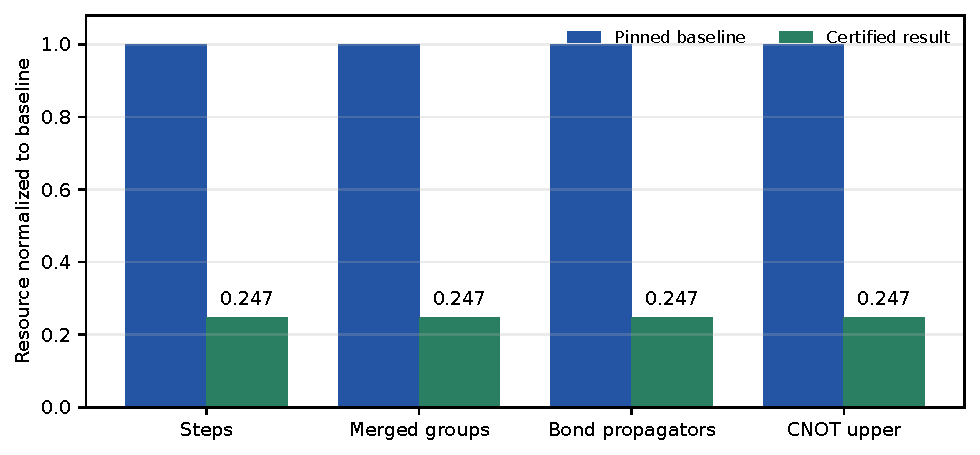
\includegraphics[width=0.94\textwidth]{figures/resources.pdf}
  \caption{Resources for the pinned theorem instantiation and the certified
  model-aware result.  Values are exact integers; axes are scaled separately
  to keep the three compiled metrics readable.}
  \label{fig:resources}
\end{figure}

\subsection{Finite-step error ledger}

At 97 steps the global upper bound is the sum of five outward rational
contributions shown in \cref{tab:error-ledger}.  The leading D4 term is only
about half the final value; D5--D7 and the tail are quantitatively material.
This demonstrates why a leading-order-only prediction would not be an
adequate certificate at the boundary.

\begin{table}[t]
\centering
\caption{Outward decimal summaries of exact rational contributions at
$r=97$.}
\label{tab:error-ledger}
\begin{tabular}{@{}lrr@{}}
\toprule
Contribution & Global error upper & Fraction of total (approx.) \\
\midrule
D4 & $5.264367936822258\times10^{-7}$ & 52.86\% \\
D5 & $1.383487536744612\times10^{-7}$ & 13.89\% \\
D6 & $1.579057000594836\times10^{-7}$ & 15.86\% \\
D7 & $1.894657080691470\times10^{-8}$ & 1.90\% \\
Tail & $1.542560312083473\times10^{-7}$ & 15.49\% \\
\midrule
Total & $9.958938494314325\times10^{-7}$ & 100\% \\
\bottomrule
\end{tabular}
\end{table}

\begin{figure}[t]
  \centering
  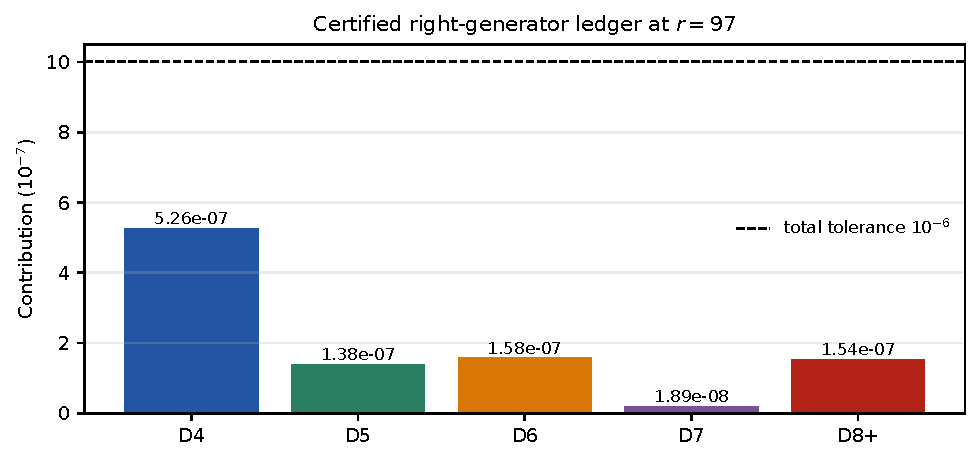
\includegraphics[width=0.72\textwidth]{figures/error_ledger.pdf}
  \caption{Finite-step error ledger at the accepted integer.  The dashed line
  marks the total tolerance, not an independent allowance for each term.}
  \label{fig:error-ledger}
\end{figure}

The adjacent-step evidence is decisive for the integer search:
97 is accepted at $9.958938494314325\times10^{-7}$, whereas the same bound at
96 evaluates to $1.050565873970784\times10^{-6}$.  The margin at 97 is about
$4.11\times10^{-9}$, so outward arithmetic and tail closure are not cosmetic;
ordinary double-precision summaries are not the source of the comparison.

\subsection{Algebraic compression statistics}

The D4 group sidecar contains 75,324 coefficient-bearing Pauli terms divided
into 7,576 verified groups.  The largest group has ten members.  The grouped
translation-cell norm $6.472926505087888$ replaces a post-aggregation direct
Pauli-$\ell_1$ value $20.160968407335066$, giving the local factor
$3.114660484942633$.  This local factor and the final resource factor need not
coincide: the latter also reflects the nonlinear inversion of the step bound,
the subleading terms, the tail, and the integer merge rule.

An auxiliary exact D5 computation produces 605,832 terms, 123,106 groups, and
a per-site upper bound $11.23706750025697$.  It is retained as evidence for a
future tightening effort.  It does not replace the complete D4--D7 global
ledger and is not used to claim a lower accepted step count.

\subsection{Small-system structural cross-check}

On a degenerate periodic $2\times2$ instance at the same 97-step count, direct
dense evaluation gives operator-norm error
$9.128277711816321\times10^{-10}$.  The schema-v3 certificate specialization
gives the upper bound $2.7666666666666666\times10^{-8}$.  The latter dominates
the measured error and remains below $10^{-6}$.  This calculation checks stage
order, normalization, periodic bookkeeping, and the direction of the
inequality using an independent dense route.  It is not an empirical proof of
the $12\times12$ result.

\subsection{Recursive Suzuki audit}

For context, the main certificate records a separate audit of standard
recursive Suzuki orders under its declared audit assumptions.  The values in
\cref{tab:recursive-audit} are taken from the manifest-bound schema-v3 JSON;
they are not used in the primary 4.05$\times$ comparison.

\begin{table}[t]
\centering
\caption{Auxiliary recursive-order audit stored in the authoritative main
certificate.}
\label{tab:recursive-audit}
\begin{tabular}{@{}rrrrr@{}}
\toprule
Order & Steps & Stages/step & Merged groups & Error upper summary \\
\midrule
2 & 29,964 & 7 & 179,785 & $9.9999203748666826\times10^{-7}$ \\
4 & 808 & 31 & 24,241 & $9.9682621337975879\times10^{-7}$ \\
6 & 370 & 151 & 55,501 & $9.8463753882538689\times10^{-7}$ \\
8 & 335 & 751 & 251,251 & $9.9829085642259163\times10^{-7}$ \\
\bottomrule
\end{tabular}
\end{table}

This audit illustrates that increasing formal order does not monotonically
reduce compiled cost at a fixed precision: the recursive stage multiplier can
outgrow the reduction in steps.  It should not be confused with a literature-
wide optimal-formula search.

\section{Related Work and Positioning}
\label{sec:related}

The relevant literature has diversified beyond a single sequence of tighter
versions of the same bound.  Some works strengthen worst-case product-formula
analysis; others restrict the state or error metric; still others change the
simulation algorithm.  A meaningful position therefore requires a taxonomy
rather than a one-dimensional ``SOTA'' label.

\subsection{Direct product-formula bounds}

Nearly optimal lattice simulation by high-order product formulas established
the favorable scaling of local formulas for geometrically local Hamiltonians
\citep{childs2019lattice}.  The commutator-scaling framework of Childs et al.
then provided general explicit error representations in terms of nested
commutators \citep{childs2021trotter}.  Model-specific evaluation has also
been developed for the Fermi--Hubbard model \citep{schubert2023hubbard}, while
strong-error analyses clarify the distinction between vector and operator
convergence for unbounded or chemistry-motivated settings
\citep{burgarth2024strong}.  Lower-bound work studies when cancellation cannot
make the Trotter error arbitrarily smaller than upper estimates
\citep{hahn2024lower}.

Our work remains in this direct, deterministic, operator-norm branch.  It does
not introduce a new asymptotic theorem.  Its contribution is an automated
finite-instance sharpening layer after the general theorem has identified the
relevant commutator structure.  The proof object retains concrete
coefficients and Pauli relations that a broad theorem cannot economically
tabulate.

\subsection{Restricted-state and average-case guarantees}

Low-energy-subspace simulation can replace global energy scales by effective
low-energy quantities when the initial state is promised to lie in an
appropriate sector \citep{sahinoglu2021lowenergy}.  Average-case analysis can
also yield speedups under distributional or norm-averaged criteria
\citep{chen2024average}.  These guarantees may be more relevant for a given
application than a worst-case operator norm, but they answer a different
question.  The present certificate makes no state promise and therefore
remains uniform over all input states.

\subsection{Changing the approximation family}

Multi-product formulas combine several product-formula circuits to cancel
leading errors.  Recent work supplies explicit commutator scaling, dynamic
coefficient selection, and time-dependent extensions
\citep{zhuk2024dynamic,aftab2024mpf,mizuta2026mpf,mizuta2026timedependent}.
Chebyshev interpolation and randomized order-doubling similarly alter how
approximants are combined \citep{rendon2024chebyshev,cho2024doubling}.
Time-dependent product-formula constructions such as THRIFT exploit an
interaction-picture decomposition \citep{bosse2025thrift}.  LCU-based Trotter
compensation and error-mitigation approaches add coherent or classical
correction layers \citep{zeng2025lcu,watson2025mitigation}; more recent nested-
commutator compensation seeks polylogarithmic precision without ancillas
\citep{wang2026hncc}.

These methods can asymptotically or practically outperform repetition of a
single deterministic Suzuki step.  Their costs include extra circuit
variants, sampling, negative or complex weights, success amplification,
ancillas, or different depth/gate accounting.  Our certified result keeps the
original formula family fixed and reduces only the justified repetition
count.  It is therefore complementary: the same proof-carrying norm compiler
could in principle supply coefficient bounds to an extrapolation or
compensation method, but such an extension is not established here.

\subsection{Formula and ordering optimization}

Optimized Trotter--Suzuki coefficient sets can lower the stage count or error
constant relative to recursive constructions \citep{malezic2026schemes}.
Commutation-aware ordering studies show that the placement of Heisenberg-type
terms can materially change realized error \citep{tate2026ordering}.
Practical error estimators trade some formal generality for computable
instance-level predictions \citep{maxwell2026practical}.  Those directions
optimize the source formula or estimate its behavior.  Here the source stage
sequence is fixed and the novelty is in rigorously compiling its complete
defect into a checkable upper bound.

\begin{table}[p]
\centering
\small
\caption{Methodological comparison.  ``Same target'' means a deterministic,
uniform operator-norm certificate for the fixed formula and compilation model
of \cref{sec:problem}.}
\label{tab:literature-map}
\begin{tabularx}{\textwidth}{@{}p{0.18\textwidth}p{0.18\textwidth}p{0.19\textwidth}p{0.18\textwidth}X@{}}
\toprule
Line of work & Main mechanism & Guarantee/cost change & Relation to our method &
Same target? \\
\midrule
Commutator scaling \citep{childs2021trotter} & General nested-commutator error
representation & Worst-case direct product formula & Supplies the pinned
control and theoretical foundation & Yes, at theorem level \\
Model-specific Hubbard bounds \citep{schubert2023hubbard} & Evaluate locality
and commutators for another model & Model-aware direct bound & Similar
model-specific philosophy; different Hamiltonian and certificate machinery &
Partly \\
Low-energy simulation \citep{sahinoglu2021lowenergy} & Restrict input energy
sector & State-dependent promise & Could be combined with concrete algebra;
not used here & No \\
Average-case speedup \citep{chen2024average} & Weaken worst-case metric to an
average & Distribution-dependent error & Orthogonal norm objective & No \\
Dynamic/explicit MPF \citep{zhuk2024dynamic,aftab2024mpf,mizuta2026mpf} &
Linear combination of several formula lengths & New coefficients, sampling or
coherent combination & Our defect bounds may inform coefficients; current
circuit family differs & No \\
Interpolation / randomization \citep{rendon2024chebyshev,cho2024doubling} &
Combine runs or random orderings & Changed estimator/algorithm & Potential
outer layer around certified formulas & No \\
THRIFT \citep{bosse2025thrift} & Time-dependent interaction-picture formula &
Changed decomposition and circuit & Could benefit from proof-carrying
instance analysis & No \\
LCU/mitigation \citep{zeng2025lcu,watson2025mitigation,wang2026hncc} & Correct
or cancel Trotter error & Ancilla, sampling, or compensation overhead & Uses
error structure actively; ours only reduces safe repetitions & No \\
Formula/ordering optimization \citep{malezic2026schemes,tate2026ordering} &
Change stages, coefficients, or ordering & Different source circuit &
Complementary front end to our compiler & No \\
This work & Complete-formula Lie extraction, exact Pauli aggregation, verified
anticommuting norms & Same formula; smaller certified repetition count &
Finite-instance proof-carrying sharpening & Yes \\
\bottomrule
\end{tabularx}
\end{table}

\subsection{Position of the present result}

Within the narrow target class, this work establishes a strong finite-instance
result: a 4.050498$\times$ certified reduction over a pinned application of a
published general theorem, while preserving the formula, operator-norm metric,
and gate-accounting rule.  Its scientific role is best described as a
\emph{model-aware proof compiler} between general theory and executable
resource estimation.

It would be inaccurate to call the result an unconditional global state of the
art in Hamiltonian simulation.  More recent algorithms can have superior
precision scaling or lower costs under changed assumptions.  Conversely,
their headline numbers do not invalidate this result because they are not
necessarily certificates for the same fixed deterministic circuit.  The
paper's defensible novelty is the combination of full-formula symbolic
cancellation, concrete Pauli norm compression, nonasymptotic closure, and an
independently checkable artifact.

\section{Limitations and Research Roadmap}
\label{sec:limitations}

The present evidence supports a precise but deliberately narrow conclusion.
This section identifies the boundaries and shows how each could be addressed
without weakening the current claim.

\subsection{Finite instance rather than universal scaling}

The numerical certificate is for the periodic $12\times12$ isotropic
Heisenberg benchmark at $T=1$ and $\eps=10^{-6}$.  Locality suggests that many
symbolic densities extend to larger tori beyond the support radius, but the
current manifest does not claim a theorem uniform in $L$, anisotropy, time, or
tolerance.  A scaling paper would require parameterized wraparound proofs,
analytic dependence of every ledger term, and certificates across a grid of
$(L,T,\eps)$ values.

\subsection{Fixed product formula and cost model}

The candidate and control use the same five-copy fourth-order Suzuki formula.
No search over modern optimized splittings is included.  Similarly, the
three-CNOT bond cost is an upper-bound compilation model, not a full
fault-tolerant resource estimate.  Native two-qubit gates, routing, parallel
depth, synthesis precision, error correction, and logical-state preparation
can change the operational optimum.  Future work should make the cost model a
pluggable certificate field and report Pareto fronts for group count, two-
qubit gates, and depth.

\subsection{Certificate size and discovery cost}

The exact D4 and D5 ledgers are large.  They are appropriate for an offline
proof artifact but not yet an interactive compiler pass.  The deep verifier is
much simpler than the generator but still scales with every listed term and
pair checked within a group.  Merkleized chunks, streaming verification,
symmetry-orbit proofs, and formally verified local rewrite kernels could
reduce storage and trust without replacing explicit evidence by an opaque
claim.

\subsection{The fivefold boundary is open}

A fivefold resource ratio would be obtained at $r=78$ because
\begin{equation}
  \frac{11{,}791}{30\cdot78+1}
  =\frac{11{,}791}{2{,}341}
  =5.036736437419906\ldots.
\end{equation}
This is arithmetic, not a 78-step error certificate.  The checked artifacts
identify three unresolved proof gates: a tighter translation-coupled D4 norm
at the 78-step budget, explicit D8 information with a delayed high-degree
tail, and a complete exact global ledger at $r=78$.  Exact D5 grouping alone
does not discharge these obligations.

\begin{figure}[t]
  \centering
  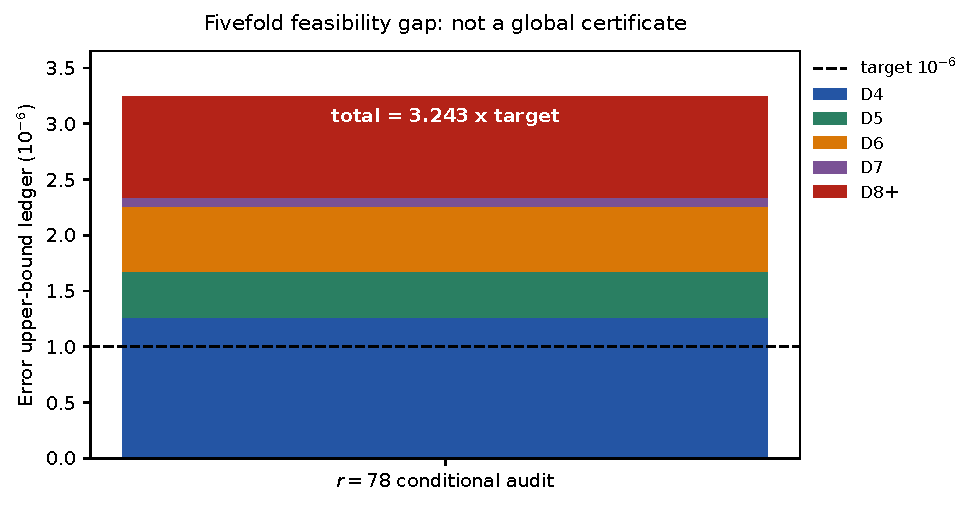
\includegraphics[width=0.8\textwidth]{figures/fivefold_gap.pdf}
  \caption{Conditional error ledger at the fivefold resource threshold.  The
  stacked value exceeds the target; $r=78$ is therefore not certified.  The
  97-step result remains the lowest accepted point of the current bound.}
  \label{fig:fivefold-gap}
\end{figure}

A disciplined optimization sequence is therefore: (1) profile the current
97-step error ledger; (2) improve the dominant D4 norm while preserving a
verifiable partition; (3) emit D8 explicitly; (4) move the geometric tail to a
higher starting degree; (5) regenerate exact contributions at 78; and (6)
accept the point only if the rational sum is at most $10^{-6}$.  GPU or HPC
parallelism can accelerate term generation and graph search, but cannot
replace the last verifier step.

\subsection{Optimality is relative to the bound}

The rejection at 96 establishes adjacent minimality only under the emitted
upper bound.  It is not a lower bound on the true operator error.  Direct
large-system matrix simulation is infeasible, and lower-bound techniques have
not been specialized here to close the gap.  Consequently the candidate may
still be physically accurate with fewer steps.  The scientific claim concerns
what can be guaranteed, not an assertion that 97 executions are necessary.

\subsection{Toward broader validation}

The most valuable next experiments are not additional decimal precision at
the current point.  They are adversarial reproductions: an independent Pauli
engine, certificates for open and periodic boundaries, anisotropic XXZ
couplings, alternate fragment orderings, and comparisons against optimized
splittings.  These tests would reveal whether the dominant gains arise from
universal compiler structure or accidental symmetries of the isotropic
benchmark.

\section{Reproducibility and Artifact Protocol}
\label{sec:reproducibility}

The repository is organized so that a reader can first validate the headline
claim in seconds and then choose progressively more expensive checks.  No
private cluster is required to verify the submitted certificate.

\subsection{Environment and commands}

The reference implementation requires Python 3.11 or later and declares
NumPy, SciPy, and SymPy dependencies.  From the \code{issue128} directory, the
standard sequence is:
\begin{verbatim}
python -m pip install -e '.[test]'
pytest -q
PYTHONPATH=src python scripts/verify.py \
  certificates/issue128-certificate.json
PYTHONPATH=src python scripts/build_d5_certificate.py --verify-only
PYTHONPATH=src python scripts/package_delivery.py --check
shasum -a 256 -c artifacts/SHA256SUMS
\end{verbatim}
The expensive algebraic replay is requested explicitly:
\begin{verbatim}
PYTHONPATH=src python scripts/verify.py \
  certificates/issue128-certificate.json --deep
\end{verbatim}
The main certificate can be regenerated with
\begin{verbatim}
PYTHONPATH=src python scripts/build_v3_certificate.py
\end{verbatim}
Long research-reproduction tests are marked \code{slow} and excluded by the
default Pytest configuration.  This separation keeps ordinary continuous
integration responsive without disguising the cost of complete regeneration.

\subsection{Claim-to-evidence map}

\begin{longtable}{@{}p{0.27\textwidth}p{0.36\textwidth}p{0.30\textwidth}@{}}
\caption{Where each principal claim is established and how it is checked.}
\label{tab:claim-map}\\
\toprule
Claim & Primary evidence & Independent check \\
\midrule
\endfirsthead
\toprule
Claim & Primary evidence & Independent check \\
\midrule
\endhead
393-step pinned control & Baseline rational and center in
\code{issue128-certificate.json} & Deep regeneration of all 31 centers \\
97 accepted, 96 rejected & Exact global and previous-step rational pairs in
the main certificate & Exact comparison against $1/10^6$ \\
75,324 D4 terms and 7,576 groups & Hashed
\code{issue128-d4-groups.json} & Coverage, symplectic pair checks, and rational
square-root replay \\
D4 bound 6.472926505087888 & Group membership and coefficient endpoints &
Verifier squares each upper root and resums \\
11,791 and 2,911 groups & Step counts plus $G(r)=30r+1$ & Direct integer
identity checks \\
Bond and CNOT totals & Cost-model fields and claimed-resource block &
$72G(r)$ and $216G(r)$ recomputation \\
4.050498$\times$ improvement & Exact pair $(11791,2911)$ & Fraction comparison,
not rounded decimal \\
Small-system consistency & Dense $2\times2$ artifact & Independent matrix
exponential and operator norm \\
D5 follow-up only & Hashed compressed D5 sidecar and summary status &
\code{--verify-only}; explicit \code{not\_certified} fivefold status \\
\bottomrule
\end{longtable}

\subsection{Immutable bindings}

At the frozen delivery point the primary digests are
\begin{align*}
\mathrm{SHA256}(\text{main certificate})
 &=\code{0a09623ce3b292a3637065c870fb3153b}\ldots,\\
\mathrm{SHA256}(\text{D4 sidecar})
 &=\code{a397414bb0229fb1ebdb38798aa781fb8}\ldots,\\
\mathrm{SHA256}(\text{D5 sidecar})
 &=\code{c5e8968a93b4497b41fe42c0e364324}\ldots.
\end{align*}
The complete 64-hex-character values are stored in the package manifest and
summary.  A printed prefix is for human orientation only; verification uses
the complete digest.

The manuscript is a derived view and is not part of the frozen proof bundle.
If the manuscript, figures, or wording changes, the mathematical claim remains
bound to the same JSON and sidecars.  Conversely, any change to a certificate
requires regeneration of its digest and all summaries that cite it.

\subsection{Machine-readable and human-readable outputs}

The delivery contains a main certificate JSON, large exact sidecars, a compact
JSON summary, a plain-text summary, verification transcript, checksums, source
code, tests, a short technical report, and this long-form manuscript.  The
machine-readable objects are authoritative for exact numerators and
denominators.  Human documents explain the method and use outward decimal
summaries; they should never be parsed as the proof source.

\subsection{Research integrity statement}

Software-assisted symbolic algebra, exact arithmetic, automated tests, and
language-model-assisted drafting were used in preparing the artifact and
manuscript.  Scientific responsibility remains with the author.  Every
headline numerical statement is checked against the frozen certificate by a
separate manuscript validation script; literature statements are cited to
their primary publications.  No generative system output is accepted as a
mathematical witness without executable or deductive verification.

\section{Conclusion}
\label{sec:conclusion}

We have presented a proof-carrying, model-aware compiler for rigorous
product-formula resource bounds.  Its central design rule is simple: preserve
algebraic structure until all formula-specific, model-specific, translational,
and anticommuting relations have been exposed; apply irreversible norm
inequalities only afterward; and emit enough evidence for an independent
program to recheck the result.

For the periodic $12\times12$ isotropic Heisenberg benchmark, this procedure
certifies the original five-copy fourth-order Suzuki circuit at 97 steps.  The
pinned general-theorem instantiation requires 393 steps under the common
comparison protocol.  After deterministic stage merging and bond
compilation, the corresponding group, bond, and CNOT resources fall by the
exact factor $11791/2911=4.050498110614909\ldots$.  The result includes the
rejected 96-step neighbor, D4--D7 contributions, a rational high-degree tail,
full D4 anticommuting membership, resource arithmetic, and hash bindings.

The broader lesson is not that one Hamiltonian has exhausted the possibilities
of Trotter simulation.  It is that a general error theorem and a concrete gate
estimate should be connected by a transparent compiler rather than a chain of
unrecorded inequalities.  The current artifact occupies that middle layer.  A
fivefold threshold remains a well-specified research target, but it will be
claimed only after the missing D4, D8, and tail obligations close in the same
machine-checkable form.


\appendix
\section{Right-Generator Expansion Details}
\label{app:right-generator}

This appendix records the finite-order identity used by the certificate.  Let
\begin{equation}
 Z(t)=\log S_4(t)=tA+t^5B+t^7C+O(t^9).
\end{equation}
Using
\begin{equation}
 \operatorname{dexp}_{Z}(Z')=
 Z'+\frac12[Z,Z']+\frac16[Z,[Z,Z']]
 +\frac1{24}[Z,[Z,[Z,Z']]]+\cdots,
\end{equation}
and collecting powers through $t^7$ gives
\begin{align}
 S_4'(t)S_4(t)^{-1}-A
  ={}&5t^4B+2t^5[A,B]
  +t^6\left(7C+\frac23[A,[A,B]]\right)\nonumber\\
  &+t^7\left(3[A,C]+\frac16[A,[A,[A,B]]]\right)
  +R_{\geq8}(t).
 \label{eq:exact-right-expansion}
\end{align}
For example, the $t^5[A,B]$ coefficient comes from
$\frac12[tA,5t^4B]+\frac12[t^5B,A]=2t^5[A,B]$.
The later coefficients follow by the same homogeneous bookkeeping.  The
implementation constructs the series in the word algebra and regression-tests
\cref{eq:exact-right-expansion}; it does not substitute the printed identity
as an unchecked constant table.

The global contribution of a monomial $t^jD_j$ follows from
\cref{eq:global-duhamel}:
\begin{equation}
 r\int_0^{T/r}s^j\opnorm{D_j}\,ds
 =\frac{T^{j+1}\opnorm{D_j}}{(j+1)r^j}.
 \label{eq:monomial-global}
\end{equation}
This explains the degree labels in the result ledger and provides a direct
dimensional check on the inverse powers of $r$.

\section{Local Heisenberg Pauli Audit}
\label{app:local-pauli}

The single-bond lemma can be checked without symbolic software.  Let
$Q_1=XX$, $Q_2=YY$, and $Q_3=ZZ$.  For a phase-free two-qubit Pauli
$P=P_1\otimes P_2$, the number of $Q_j$ that anticommute with $P$ is either
zero or two.  One compact enumeration is shown in \cref{tab:local-audit}; rows
and columns give the one-qubit factors.

\begin{table}[ht]
\centering
\caption{Number of anticommuting terms among $XX,YY,ZZ$ for every local
two-qubit Pauli.}
\label{tab:local-audit}
\begin{tabular}{@{}c|rrrr@{}}
\toprule
$P_1\backslash P_2$ & $I$ & $X$ & $Y$ & $Z$ \\
\midrule
$I$ & 0 & 2 & 2 & 2 \\
$X$ & 2 & 0 & 2 & 2 \\
$Y$ & 2 & 2 & 0 & 2 \\
$Z$ & 2 & 2 & 2 & 0 \\
\bottomrule
\end{tabular}
\end{table}

If the count is zero, $[h,P]=0$.  If it is two, each contributing Hamiltonian
coefficient has magnitude $1/4$ and the Pauli commutator supplies magnitude
two, giving two output coefficients of magnitude $1/2$.  Their
Pauli-$\ell_1$ sum is one.  Hence
\begin{equation}
  \paulinorm{[h,P]}\leq1=\paulinorm{P}
\end{equation}
for a unit Pauli input, and linearity extends the stated growth majorant.  The
generic bound obtained by summing the three Hamiltonian Paulis independently
would give $3/2$; the exact parity enumeration removes the impossible third
contribution.

\section{Verifier Pseudocode}
\label{app:verifier}

\begin{algorithm}[ht]
\caption{Independent verification of the principal certificate}
\label{alg:verifier}
\begin{algorithmic}[1]
\Require main certificate $C$ and sidecar directory
\State validate schema version and required benchmark fields
\State recompute SHA-256 for every referenced sidecar
\State verify formula, normalization, $T$, $\eps$, and cost-model identities
\State load the D4 coefficient ledger and declared group partition
\State verify exact coverage: no missing, duplicate, or unknown Pauli key
\For{every group $G$}
  \For{every unordered pair $(P,Q)\subseteq G$}
    \State require symplectic parity$(P,Q)=1$
  \EndFor
  \State recompute the rational squared-weight sum
  \State require declared upper root squared $\geq$ recomputed sum
\EndFor
\State sum all group roots and compare to the D4 cell enclosure
\State verify D5--D7 and tail preconditions and contributions
\State sum the accepted-step global rational; require result $\leq\eps$
\State sum the previous-step rational; require result $>\eps$
\State recompute $G(r)$, bond propagators, CNOT totals, and exact ratio
\State return a structured success record; fail closed on any mismatch
\end{algorithmic}
\end{algorithm}

Deep mode inserts regeneration of the baseline center scan, complete formula
logarithm, DSW defects, Pauli coefficient map, and higher-degree majorants
before the certificate comparisons.  Importantly, both modes fail closed:
unknown schema versions, absent files, extra group members, and invalid
interval orientation are errors rather than warnings.

\section{Certificate Schema Sketch}
\label{app:schema}

\begin{longtable}{@{}p{0.29\textwidth}p{0.19\textwidth}p{0.44\textwidth}@{}}
\caption{Selected schema-v3 fields and verification obligations.}
\label{tab:schema}\\
\toprule
Field & Type & Obligation \\
\midrule
\endfirsthead
\toprule
Field & Type & Obligation \\
\midrule
\endhead
\path{benchmark} & object & Exact model, normalization, size, time,
tolerance, and primary metric match the claim \\
\path{published_baseline.site_density_upper} & integer pair & Denominator is
positive and deep regeneration is enclosed \\
\path{candidate.d4_certificate.path} & relative path & Resolves inside the
bundle; no path traversal \\
\path{candidate.d4_certificate.sha256} & 64-hex digest & Equals the bytes of
the resolved sidecar \\
\path{candidate.contributions} & rational pairs & Each pair has positive
denominator and agrees with recomputed bounds \\
\path{candidate.global_error_upper} & rational pair & Equals or dominates
the contribution sum and is below tolerance \\
\path{candidate.previous_step_error_upper} & rational pair & Correctly
evaluated at $r-1$ and exceeds tolerance \\
\path{cost_model} & integers/rule & Resource identities are evaluated without
floating point \\
\path{claimed_resources} & integer object & Every total is reconstructed from
the step count and cost model \\
\path{claims.exact_improvement_ratio} & integer pair & Equals the declared
baseline and candidate group counts \\
\bottomrule
\end{longtable}

\section{Additional Interpretation of the Improvement}
\label{app:interpretation}

Several ratios appear in the analysis and should not be conflated:
\begin{align}
\text{D4 norm tightening}
  &=\frac{20.160968407335066}{6.472926505087888}
    =3.114660484942633\ldots,\\
\text{step ratio}
  &=\frac{393}{97}=4.051546391752577\ldots,\\
\text{compiled resource ratio}
  &=\frac{30\cdot393+1}{30\cdot97+1}
    =\frac{11791}{2911}
    =4.050498110614909\ldots.
\end{align}
The step and resource ratios differ because the first and last fragment groups
merge to give the additive one in \cref{eq:merged-groups}.  The norm ratio is
not expected to equal either: a fourth-order global error scales roughly as
$r^{-4}$ only in a leading asymptotic regime, while the actual accepted point
contains D5--D7, a tail, and integer rounding.

The improvement relative to the challenge's twofold target is
\begin{equation}
 \frac{(11791/2911)}{2}=2.025249055307454\ldots.
\end{equation}
This means the achieved multiplier is just over twice the requested
multiplier; it does not mean an eightfold resource reduction.

\section{Checklist for Independent Review}
\label{app:checklist}

A reviewer can audit the result in increasing order of cost:
\begin{enumerate}
\item Read the benchmark tuple and confirm that candidate and control use the
same Hamiltonian, formula, tolerance, and cost model.
\item Run the manuscript headline validator and the package checksum check.
\item Run the fast verifier and inspect its structured output.
\item Confirm the exact integer map from 393/97 steps to all three resources.
\item Run the default unit suite, including mutation and local-Pauli tests.
\item Run D5 \code{--verify-only} to confirm the follow-up is separate and
marked noncertified at 78 steps.
\item If computational resources permit, run the deep verifier to regenerate
the formula-specific algebra and baseline center scan.
\item Rebuild this PDF and visually inspect figures, tables, citations, and
page boundaries; PDF appearance is a communication check, not a proof check.
\end{enumerate}


{\small
\bibliographystyle{unsrtnat}
\bibliography{references}
}
\end{document}
